\section{HOLD Plot Hold Toggle Function}

\subsection{Usage}

Toggles the hold state on the currently active plot.  The
general syntax for its use is
\begin{verbatim}
   hold(state)
\end{verbatim}
where \verb|state| is either
\begin{verbatim}
   hold('on')
\end{verbatim}
to turn hold on, or
\begin{verbatim}
   hold('off')
\end{verbatim}
to turn hold off. If you specify no argument then
\verb|hold| toggles the state of the hold:
\begin{verbatim}
   hold
\end{verbatim}
You can also specify a particular axis to the hold command
\begin{verbatim}
   hold(handle,...)
\end{verbatim}
where \verb|handle| is the handle for a particular axis.
\subsection{Function Internals}

The \verb|hold| function allows one to construct a plot sequence
incrementally, instead of issuing all of the plots simultaneously
using the \verb|plot| command.
\subsection{Example}

Here is an example of using both the \verb|hold| command and the
multiple-argument \verb|plot| command to construct a plot composed
of three sets of data.  The first is a plot of a modulated Gaussian.
\begin{verbatim}
--> x = linspace(-5,5,500);
--> t = exp(-x.^2);
--> y = t.*cos(2*pi*x*3);
--> plot(x,y);
\end{verbatim}


\centerline{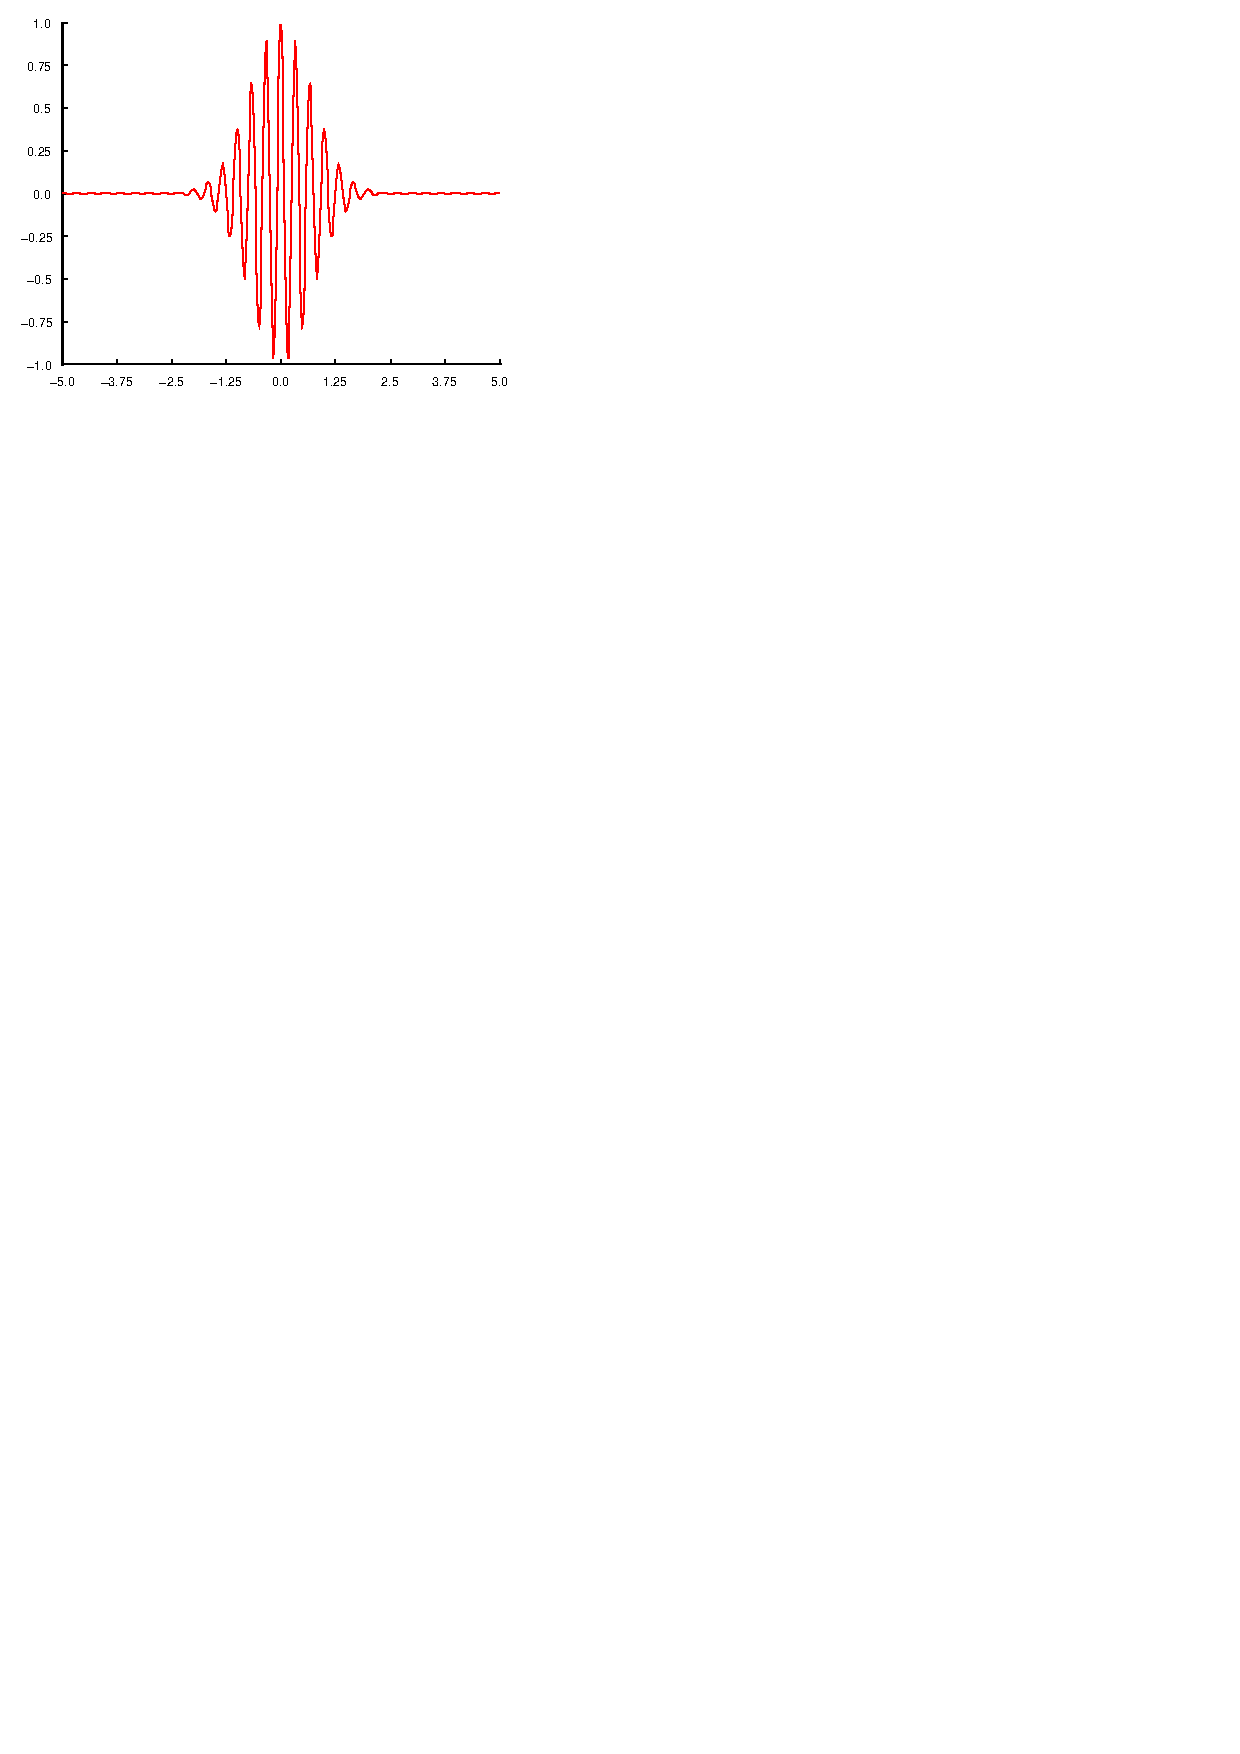
\includegraphics[width=8cm]{hold1}}


We now turn the hold state to \verb|'on'|, and add another plot
sequence, this time composed of the top and bottom envelopes of
the modulated Gaussian.  We add the two envelopes simultaneously
using a single \verb|plot| command.  The fact that \verb|hold| is
\verb|'on'| means that these two envelopes are added to (instead of
replace) the current contents of the plot.
\begin{verbatim}
--> plot(x,y);
--> hold on
--> plot(x,t,'g-',x,-t,'b-')
\end{verbatim}


\centerline{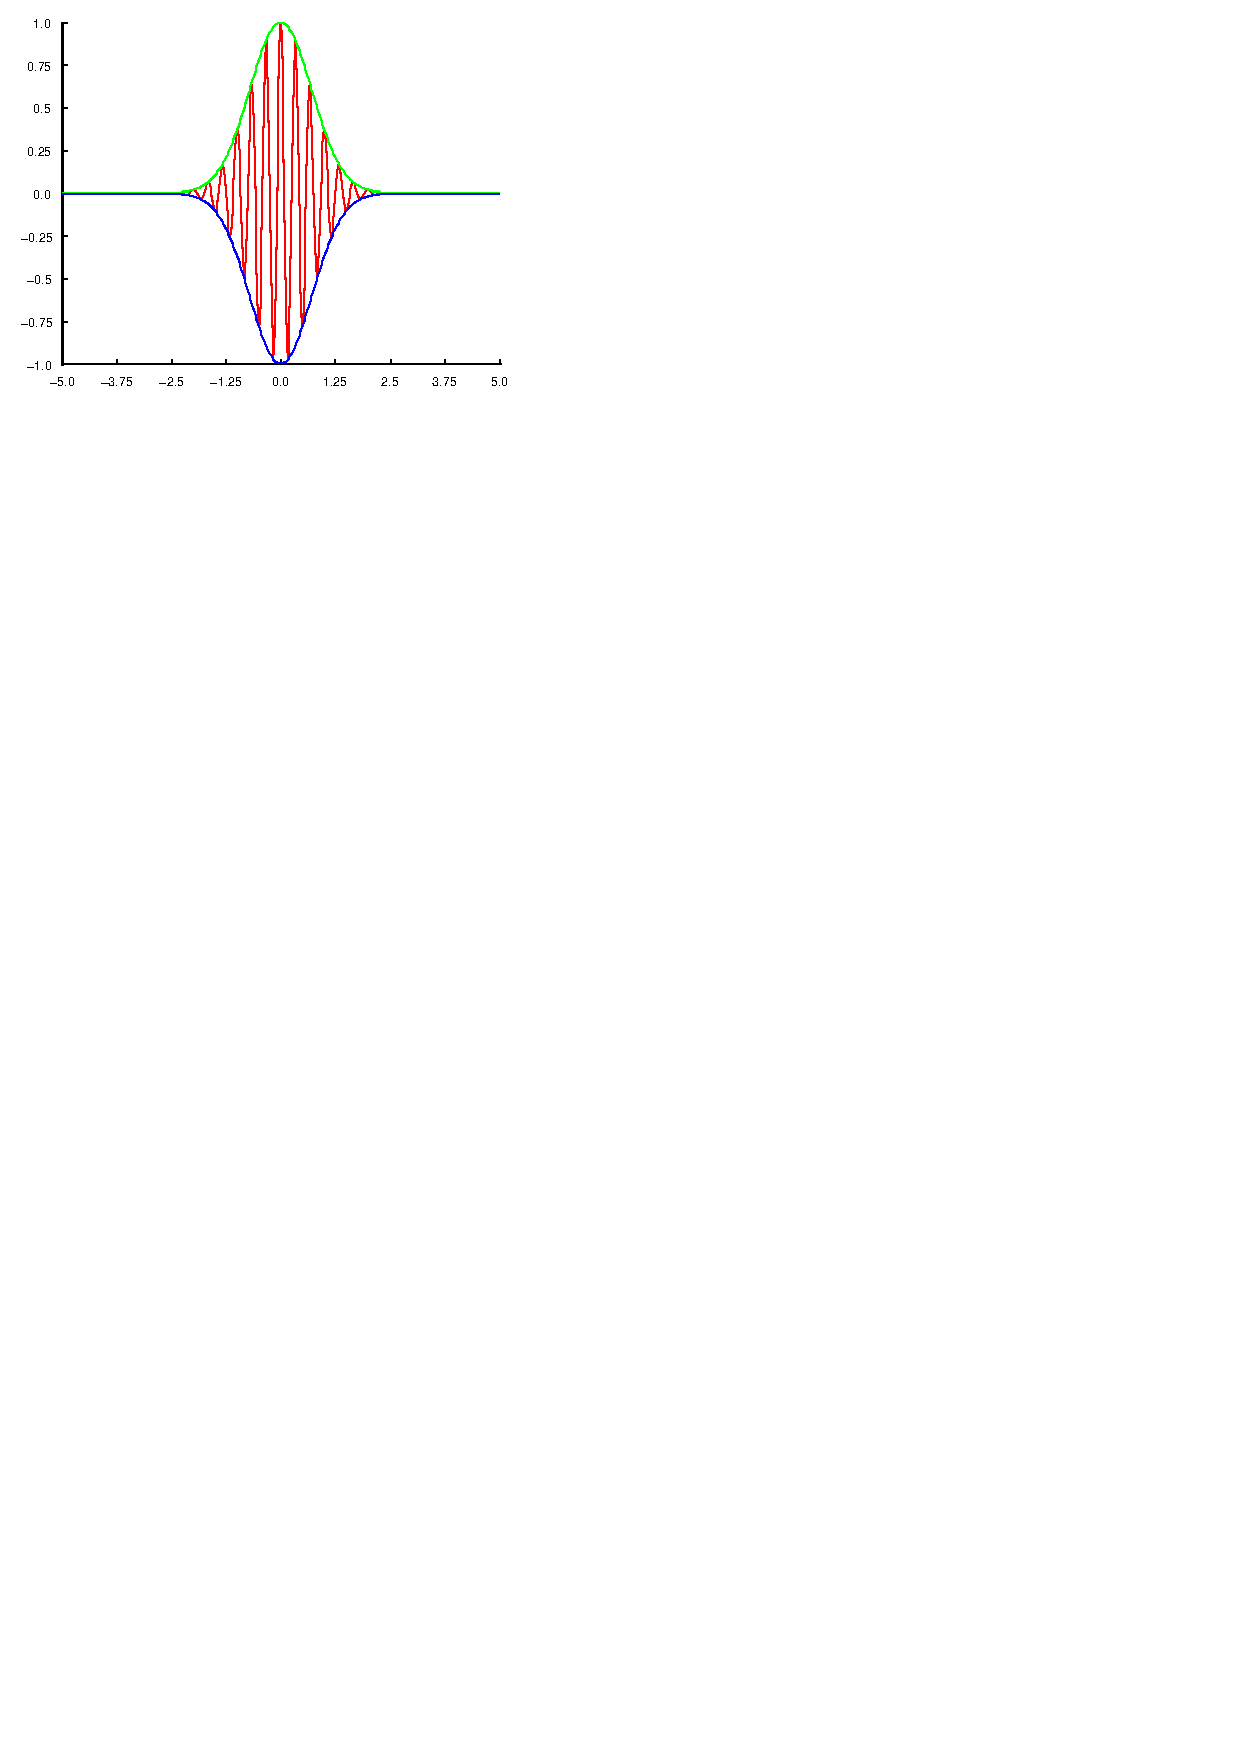
\includegraphics[width=8cm]{hold2}}

